\documentclass{article}
\usepackage[utf8]{inputenc}
\usepackage{amsmath, amssymb, systeme, mathtools, lmodern, float, graphicx}
\usepackage[most]{tcolorbox}
\usepackage[scale=.95,type1]{cabin}
\usepackage[framemethod=tikz]{mdframed}

\usepackage[legalpaper,margin=1in]{geometry}

\setlength{\parindent}{10pt}
\setlength{\parskip}{1em}
\renewcommand{\baselinestretch}{1.2}

\title{Chapter 7: Eigenvalues and Eigenvectors}
\date{}

\makeatletter
\renewcommand*\env@matrix[1][*\c@MaxMatrixCols c]{%
  \hskip -\arraycolsep
  \let\@ifnextchar\new@ifnextchar
  \array{#1}}
\makeatother

\newcommand\y{\cellcolor{blue!10}}

\usepackage{tabularray}
\SetTblrInner{colsep=5pt,rowsep=1pt}

\newcommand\x{\times}
\newcommand\xor{\oplus}

\makeatletter
\newcommand{\dashover}[2][\mathop]{#1{\mathpalette\df@over{{\dashfill}{#2}}}}
\newcommand{\fillover}[2][\mathop]{#1{\mathpalette\df@over{{\solidfill}{#2}}}}
\newcommand{\df@over}[2]{\df@@over#1#2}
\newcommand\df@@over[3]{%
  \vbox{
    \offinterlineskip
    \ialign{##\cr
      #2{#1}\cr
      \noalign{\kern1pt}
      $\m@th#1#3$\cr
    }
  }%
}
\newcommand{\dashfill}[1]{%
  \kern-.5pt
  \xleaders\hbox{\kern.5pt\vrule height.4pt width \dash@width{#1}\kern.5pt}\hfill
  \kern-.5pt
}
\newcommand{\dash@width}[1]{%
  \ifx#1\displaystyle
    2pt
  \else
    \ifx#1\textstyle
      1.5pt
    \else
      \ifx#1\scriptstyle
        1.25pt
      \else
        \ifx#1\scriptscriptstyle
          1pt
        \fi
      \fi
    \fi
  \fi
}
\newcommand{\solidfill}[1]{\leaders\hrule\hfill}
\makeatother

\newcommand\R{\mathbb{R}}

\DeclarePairedDelimiter\abs{\lvert}{\rvert}%
\DeclarePairedDelimiter\norm{\lVert}{\rVert}%

% Swap the definition of \abs* and \norm*, so that \abs
% and \norm resizes the size of the brackets, and the 
% starred version does not.
\makeatletter
\let\oldabs\abs
\def\abs{\@ifstar{\oldabs}{\oldabs*}}
%
\let\oldnorm\norm
\def\norm{\@ifstar{\oldnorm}{\oldnorm*}}
\makeatother

\newcommand*{\Value}{\frac{1}{2}x^2}%

\newcommand\ddfrac[2]{\frac{\displaystyle #1}{\displaystyle #2}}


\newcounter{Theo}[section]
\newenvironment{Theo}[1][]{%
  \stepcounter{Lemma}%
  \ifstrempty{#1}%
  {\mdfsetup{%
    frametitle={%
      \tikz[baseline=(current bounding box.east),outer sep=0pt]
      \node[line width=1pt,anchor=east,rectangle,draw=blue!20,fill=white]
    {\strut \color{black}{\textit{THEOREM}}~};}}
  }%
  {\mdfsetup{%
    frametitle={%
      \tikz[baseline=(current bounding box.east),outer sep=0pt]
      \node[line width=1pt,anchor=east,rectangle,draw=blue!20,fill=white]
    {\strut \color{black}{\textit{THEOREM}}~:~\color{blue5}{#1}};}}%
  }%
  \mdfsetup{innertopmargin=10pt,linecolor=blue!20,%
            linewidth=1pt,topline=true,%
            frametitleaboveskip=\dimexpr-\ht\strutbox\relax,}
  \begin{mdframed}[]\relax%
  }{\end{mdframed}}

\newcounter{Def}[section]
\newenvironment{Def}[1][]{%
  \ifstrempty{#1}%
  {\mdfsetup{%
    frametitle={%
      \tikz[baseline=(current bounding box.east),outer sep=0pt]
      \node[line width=1pt,anchor=east,rectangle,draw=blue!20,fill=white]
    {\strut \color{black}{Definition}~};}}
  }%
  {\mdfsetup{%
    frametitle={%
      \tikz[baseline=(current bounding box.east),outer sep=0pt]
      \node[line width=1pt,anchor=east,rectangle,draw=blue!20,fill=white]
    {\strut \color{black}{Definition}~:~\color{blue4}{#1}};}}%
  }%
  \mdfsetup{innertopmargin=2pt,linecolor=blue!20,%
            linewidth=1pt,topline=true,%
            frametitleaboveskip=\dimexpr-\ht\strutbox\relax,}
  \begin{mdframed}[]\relax%
  }{\end{mdframed}}

\newcounter{Ans}[section]
\newenvironment{Ans}[1][]{%
  \ifstrempty{#1}%
  {\mdfsetup{%
    frametitle={%
      \tikz[baseline=(current bounding box.east),outer sep=0pt]
      \node[line width=1pt,anchor=east,rectangle,draw=blue!20,fill=white]
    {\strut \color{black}{\textit{ANSWER}}~};}}
  }%
  {\mdfsetup{%
    frametitle={%
      \tikz[baseline=(current bounding box.east),outer sep=0pt]
      \node[line width=1pt,anchor=east,rectangle,draw=blue!20,fill=white]
    {\strut \color{black}{\textit{ANSWER}}~:~\color{blue4}{#1}};}}%
  }%
  \mdfsetup{innertopmargin=2pt,linecolor=blue!20,%
            linewidth=1pt,topline=true,%
            frametitleaboveskip=\dimexpr-\ht\strutbox\relax,}
  \begin{mdframed}[]\relax%
  }{\end{mdframed}}

\newcounter{Ques}[section]
\newenvironment{Ques}[1][]{%
  \ifstrempty{#1}%
  {\mdfsetup{%
    frametitle={%
      \tikz[baseline=(current bounding box.east),outer sep=0pt]
      \node[line width=1pt,anchor=east,rectangle,draw=blue!20,fill=white]
    {\strut \color{blue5}{\textit{QUESTION}}~};}}
  }%
  {\mdfsetup{%
    frametitle={%
      \tikz[baseline=(current bounding box.east),outer sep=0pt]
      \node[line width=1pt,anchor=east,rectangle,draw=blue!20,fill=white]
    {\strut \color{black}{\textit{ANSWER}}~:~\color{blue4}{#1}};}}%
  }%
  \mdfsetup{innertopmargin=2pt,linecolor=blue!20,%
            linewidth=1pt,topline=true,%
            frametitleaboveskip=\dimexpr-\ht\strutbox\relax,}
  \begin{mdframed}[]\relax%
  }{\end{mdframed}}


\newcounter{Conc}[section]
\newenvironment{Conc}[1][]{%
  \ifstrempty{#1}%
  {\mdfsetup{%
    frametitle={%
      \tikz[baseline=(current bounding box.east),outer sep=0pt]
      \node[line width=1pt,anchor=east,rectangle,draw=blue!20,fill=white]
    {\strut \color{blue5}{Conclude}~};}}
  }%
  {\mdfsetup{%
    frametitle={%
      \tikz[baseline=(current bounding box.east),outer sep=0pt]
      \node[line width=1pt,anchor=east,rectangle,draw=blue!20,fill=white]
    {\strut \color{black}{\textit{ANSWER}}~:~\color{blue4}{#1}};}}%
  }%
  \mdfsetup{innertopmargin=0pt,linecolor=blue!20,%
            linewidth=1pt,topline=true,%
            frametitleaboveskip=\dimexpr-\ht\strutbox\relax,}
  \begin{mdframed}[]\relax%
  }{\end{mdframed}}

\newcounter{Summarize}[section]
\newenvironment{Summarize}[1][]{%
  \ifstrempty{#1}%
  {\mdfsetup{%
    frametitle={%
      \tikz[baseline=(current bounding box.east),outer sep=0pt]
      \node[line width=1pt,anchor=east,rectangle,draw=blue!20,fill=white]
    {\strut \color{blue5}{\textit{SUMMARY}}~};}}
  }%
  {\mdfsetup{%
    frametitle={%
      \tikz[baseline=(current bounding box.east),outer sep=0pt]
      \node[line width=1pt,anchor=east,rectangle,draw=blue!20,fill=white]
    {\strut \color{black}{\textit{SUMMARY}}~:~\color{blue4}{#1}};}}%
  }%
  \mdfsetup{innertopmargin=0pt,linecolor=blue!20,%
            linewidth=1pt,topline=true,%
            frametitleaboveskip=\dimexpr-\ht\strutbox\relax,}
  \begin{mdframed}[]\relax%
  }{\end{mdframed}}



\begin{document}
    \part{Eigenvalues and Eigenvectors}
    \begin{Def}[Eigenvalue and Eigenvector]
        Let $A$ be an $n \times n$ matrix. The scalar $\lambda$ is called an \textbf{eigenvalue} of $A$ if there is a \textit{nonzero} vector
        \textbf{x} such that
        \[A \textbf{x} = \lambda \textbf{x}\]
        The vector \textbf{x} is called an \textbf{eigenvector} of $A$ corresponding to $\lambda$.
    \end{Def}
    \textbf{Example 1. \textcolor{blue5}{Verifying Eigenvalues and Eigenvectors}}

    For the matrix \[A = \begin{bmatrix}
        2 & 0 \\
        0 & -1
    \end{bmatrix},\]
    $ \textbf{x}_1 = (1,0)$ is an eigenvector of $A$ corresponding to the eigenvalue $\lambda_1 = 2$, and $ \textbf{x}_2 = 
    (0,1)$ is an eigenvector of $A$ corresponding to the eigenvalue $\lambda_2 = -1$.

    \textbf{Example 2. \textcolor{blue5}{Verifying Eigenvalues and Eigenvectors}}

    For the matrix \[A =
        \begin{bmatrix}
        1 & -2 & 1 \\
        0 & 0 & 0 \\
        0 & 1 & 1
    \end{bmatrix},  \]
    find the eigenvalues corresponding to these eigenvectors
    \[ \textbf{x}_1 = (-3, -1, 1) \quad \text{and} \quad \textbf{x}_2 = (1,0,0) \]
    \textit{\textcolor{blue5}{SOLUTION.}} Multiplying these vectors by $A$ produces
    \[A \textbf{x}_1 = \begin{bmatrix}
        1 & -2 & 1 \\
        0 & 0 & 0 \\
        0 & 1 & 1
    \end{bmatrix} \begin{bmatrix}
        -3 \\ -1 \\ 1
    \end{bmatrix} = \begin{bmatrix}
        0 \\ 0 \\ 0 
    \end{bmatrix} = 0 \begin{bmatrix}
        -3 \\ -1 \\ 1
    \end{bmatrix}\]
    So, $ \textbf{x}_1 = (-3,-1,1)$ is an eigenvector corresponding to the eigenvalue $\lambda_1 = 0$.
    \[A \textbf{x}_2 = \begin{bmatrix}
        1 & -2 & 1 \\
        0 & 0 & 0 \\
        0 & 1 & 1
    \end{bmatrix} \begin{bmatrix}
       1 \\ 0 \\ 0 
    \end{bmatrix} = \begin{bmatrix}
        1 \\ 0 \\ 0 
    \end{bmatrix} = 1 \begin{bmatrix}
        1 \\ 0 \\ 0
    \end{bmatrix}\]
    So, $ \textbf{x}_2 = (1,0,0)$ is an eigenvector corresponding to the eigenvalue $\lambda_2 = 1$.

    \section{Eigenspaces}
    In fact, if $A$ is an $n \times n$ matrix with an eigenvalue $\lambda$ and a corresponding eigenvector \textbf{x}, then every 
    nonzero scalar multiple of \textbf{x} is also an eigenvector of $A$. 
    \[A(c \textbf{x}) = c(A \textbf{x}) = c( \lambda \textbf{x} ) = \lambda (c \textbf{x}) \]
    It is also true that if $ \textbf{x}_1$ and $ \textbf{x}_2$ are eigenvectors corresponding to the same 
    eigenvalue $\lambda$, then their sum is also an eigenvector corresponding to $\lambda$.
    \[A( \textbf{x}_1 + \textbf{x}_2 ) = A \textbf{x}_1 + A \textbf{x}_2 = \lambda  \textbf{x}_1 + \lambda \textbf{x}_2 = \lambda( \textbf{x}_1 + \textbf{x}_2 ) \]
    \begin{tcolorbox}[colback = {blue9}]
        \textit{THEOREM 7.1} \textbf{Eigenvectors of $ \lambda$ Form a Subspace}

        If $A$ is an $n \times n$ matrix with an eigenvalue $ \lambda$, then the set of all eigenvectors of $ \lambda$, together
        with the zero vector
        \[\{ \textbf{0} \} \cup \{ \textbf{x}: \textbf{x} \text{ is an eigenvector of } \lambda\} ,\]
        is a subspace of $ \R^n $. This subspace is called the \textbf{eigenspace} of $ \lambda$.
    \end{tcolorbox}
    \textbf{Example 3. \textcolor{blue5}{An Example of Eigenspaces in the Plane}}

    Find the eigenvalues and corresponding eigenspaces of 
    \[A = \begin{bmatrix}
        -1 & 0 \\
        0 & 1
    \end{bmatrix}\]
    \textit{\textcolor{blue5}{SOLUTION.}} Geometrically, multiplying a vector  $ \textbf{v} = (x,y)$ in $ \R^2 $ by $A$   corresponds
    to a reflection in the $y$-axis.
    \[A \textbf{v} = \begin{bmatrix}
        -1 & 0 \\
        0 & 1
    \end{bmatrix} \begin{bmatrix}
        x \\ y
    \end{bmatrix} = \begin{bmatrix}
        -x \\ y
    \end{bmatrix} \]

    \begin{minipage}{0.28\linewidth}
        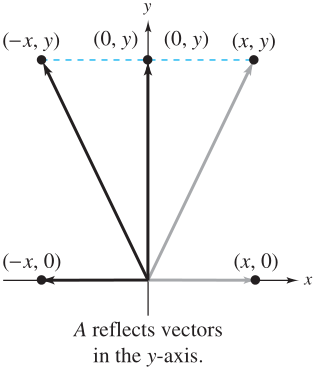
\includegraphics[width = 4cm]{images/reflection.png}
    \end{minipage}
    \begin{minipage}{0.67\linewidth}
        Notice that only vectors reflected onto scalar multiples of themselves are those lying on 
        either the $x$-axis or the $y$-axis.
        \begin{center}
            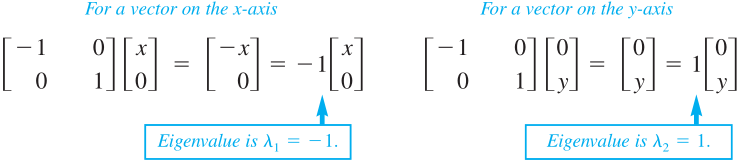
\includegraphics[width = 10cm]{images/reflection2.png}
        \end{center}
        This implies that, the eigenspace corresponding to $\lambda_1 = -1$ is the $x$-axis and the eigenspace corresponding
        to $\lambda_2 = 1$ is the $y$-axis.
    \end{minipage}

    \section{Finding Eigenvalues and Eigenvectors}
    \begin{tcolorbox}[colback = {blue9}]
        \textit{THEOREM 7.2} \textbf{Eigenvalues and Eigenvectors of a Matrix}

        Let $A$ be an $n \times n$ matrix.
        \begin{enumerate}
            \item An eigenvalue of $A$ is a scalar $ \lambda$ such that
                \[\text{det}( \lambda I - A ) = 0\]
            \item The eigenvectors of $A$ corresponding to $ \lambda$ are the nonzero solution of 
                \[( \lambda I - A ) \textbf{x} = \textbf{0}\]
        \end{enumerate}
    \end{tcolorbox}
    The equation $\text{det}(\lambda I - A) = 0$ is called the \textbf{characteristic equation} of $A$. Moreover, when expanded to
    polynomial 
    \[| \lambda I - A | = \lambda^n + c_{n-1} \lambda^{n-1} + \cdots + c_1 \lambda + c_0\]
    is called the \textbf{characteristic polynomial} of $A$. This tells us that the eigenvalues of an $n \times n$ matrix $A$ 
    correspond to the roots of the characteristic polynomial of $A$. Because the characteristic polynomial of $A$
    is of degree $n$, $A$ can have at most $n$ distinct eigenvalues.

    \textbf{Example 4. \textcolor{blue5}{Finding Eigenvalues and Eigenvectors}}

    Find the eigenvalues and corresponding eigenvectors of 
    \[A = \begin{bmatrix}
        2 & -12\\
        1 & -5
    \end{bmatrix}\]
    \textit{\textcolor{blue5}{SOLUTION.}} The characteristic polynomial of $A$ is
    \begin{equation*}
        \begin{split}
            | \lambda I - A | &= \begin{vmatrix}
                \lambda - 2 & 12\\
                -1 & \lambda + 5
            \end{vmatrix} \\
                              &= ( \lambda - 2 )( \lambda + 5 ) + 12 \\
                              &= \lambda^2 + 3 \lambda + 2 \\
                              &= ( \lambda + 1 )( \lambda +2 )
        \end{split}
    \end{equation*}
    So, the characteristic equation is $( \lambda + 1 )( \lambda + 2 ) = 0$, which gives $ \lambda_1 = -1$ and $ \lambda_2 = -2$ as the eigenvalues
    of $A$. Next, solve the homogeneous linear system $( \lambda I - A ) \textbf{x} = \textbf{0}$.

    $\bullet$ For $\lambda_1 = -1$, the coefficient matrix after row reducing is $ \begin{bmatrix}
        1 & -4 \\ 0 & 0
    \end{bmatrix}$, showing that $x_1 - 4x_2 = 0$. Letting $x_2 = t$, we can conclude that every eigenvector of $\lambda_1$
    is of the form
    \[ \textbf{x} = \begin{bmatrix}
        x_1 \\ x_2
    \end{bmatrix} = \begin{bmatrix}
        4t \\ t
    \end{bmatrix} = t \begin{bmatrix}
        4 \\ 1
    \end{bmatrix}, t \ne 0\]

    $\bullet$ For $\lambda_2 = -2$, the coefficient matrix after row reducing is $ \begin{bmatrix}
        1 & -3 \\ 0 & 0
    \end{bmatrix}$, showing that $x_1 - 3x_2 = 0$. Letting $x_2 = t$, we can conclude that every eigenvector of $\lambda_1$
    is of the form
    \[ \textbf{x} = \begin{bmatrix}
        x_1 \\ x_2
    \end{bmatrix} = \begin{bmatrix}
        3t \\ t
    \end{bmatrix} = t \begin{bmatrix}
        3 \\ 1
    \end{bmatrix}, t \ne 0\]

    \begin{Summarize}[Finding Eigenvalues and Eigenvectors]
        Let $A$ be an $n \times n$ matrix.\\
        1. Form the characteristic equation $| \lambda I - A| = 0$, which is a polynomial equation of degree $n$ in the variable $ \lambda$.\\
        2. Find the real roots of the characteristic equation. These are the eigenvalues of $A$. \\
        3. For each eigenvalue $\lambda_i$, find the corresponding eigenvectors by solving the homogeneous system
        \[( \lambda_i I  - A ) \textbf{x} = \textbf{0} \]
    \end{Summarize}

    \textbf{Example 5. \textcolor{blue5}{Finding Eigenvalues and Eigenvectors}}

    Find the eigenvalues and corresponding eigenvectors of
    \[A = \begin{bmatrix}
        2 & 1 & 0 \\
        0 & 2 & 0 \\
        0 & 0 & 2
    \end{bmatrix}\]
    What is the dimension of the eigenspace of each eigenvalues?

    \textit{\textcolor{blue5}{SOLUTION.}} The characteristic polynomial of $A$ is
    \[| \lambda I - A| =  \begin{vmatrix}
        \lambda - 2  & -1 & 0 \\
        0 & \lambda - 2 & 0 \\
        0 & 0 & \lambda - 2
    \end{vmatrix} = ( \lambda - 2 )^3 \]
    So, the characteristic equation is $( \lambda - 2 )^3 = 0$. Thus, the only eigenvalue is $ \lambda = 2$.

    \[ \lambda I - A = 2I - A = \begin{bmatrix}
        0 & -1 & 0 \\
        0 & 0 & 0 \\
        0 & 0 & 0
    \end{bmatrix}\]
    This implies that $x_2 = 0$. Using the parameters $s = x_1$ and $t = x_3$, we can find that the eigenvectors of 
    $ \lambda = 2$ are of the form
    \[ \textbf{x} = \begin{bmatrix}
        x_1 \\ x_2 \\ x_3 
    \end{bmatrix} = \begin{bmatrix}
        s \\ 0 \\ t
    \end{bmatrix} = s \begin{bmatrix}
        1 \\ 0 \\ 0
    \end{bmatrix} + t \begin{bmatrix}
        0 \\ 0 \\ 1
    \end{bmatrix}, \text{$s$ and $t$ not both zero.} \]
    Because $ \lambda = 2$ has 2 linearly independent eigenvectors, the dimension of its eigenspace is 2.

    {\color{blue9} \rule{10cm}{0.3mm}}

    If an eigenvalue $ \lambda _1$ occurs as a \textit{multiple root} ($k$ times) of the characteristic polynomial, then $ \lambda _1$ has \textbf{multiplicity} $k$.
    This implies that $( \lambda  - \lambda _1 )^k$ is a factor of the characteristic polynomial and $( \lambda  - \lambda _1 )^{k+1}$ is not. 

    For instance,
    in Example 5 the eigenvalue $ \lambda  = 2$ has a multiplicity of $3$. Also note that, the \textbf{dimension} of the eigenspace of $ \lambda  = 2$ is 2.
    In general, the \textit{multiplicity} of $ \lambda_i$ is greater than or equal to the \textit{dimension} of its eigenspace. 
    \textcolor{blue5}{(Tell me if you want a proof)}

    \textbf{Example 6. \textcolor{blue5}{Finding Eigenvalues and Eigenvectors}}

    Find the eigenvalues of
    \[A = \begin{bmatrix}[rrrr]
        1 & 0 & 0 & 0 \\
        0 & 1 & 5 & -10 \\
        1 & 0 & 2 & 0\\
        1 & 0 & 0 & 3
    \end{bmatrix} \]
    and find a basis for each of the corresponding eigenspaces.
    
    \textit{\textcolor{blue5}{SOLUTION.}} The characteristic polynomial of $A$ is 
    \begin{equation*}
        \begin{split}
            | \lambda  I - A| &= \begin{bmatrix}[rrrr]
        \lambda  - 1 & 0 & 0 & 0 \\
        0 & \lambda  - 1 & -5 & 10 \\
        -1 & 0 & \lambda  -2 & 0\\
        -1 & 0 & 0 & \lambda  -3
    \end{bmatrix} \\
    &= ( \lambda  - 1 )^2( \lambda  - 2 )( \lambda -3 )
        \end{split}
    \end{equation*}
    So, the eigenvalues are $\lambda_1 = 1$, $\lambda_2 = 2$ and $ \lambda _3 = 3$. (Note that $ \lambda _1$ has a multiplicity of 2.)
    
    $\bullet$ For $\lambda_1 = 1$:
    \[(1)I - A = \begin{bmatrix}[rrrr]
        0 & 0 & 0 & 0 \\
        0 & 0 & -5 & 10\\
        -1 & 0 & -1 & 0 \\
        -1 & 0 & 0 & -2
    \end{bmatrix} \implies \begin{bmatrix}[rrrr]
        1 & 0 & 0 & 2 \\
        0 & 0 & 1 & -2 \\
        0 & 0 & 0 & 0 \\
        0 & 0 & 0 & 0 
    \end{bmatrix} \]
    Letting $s = x_2$ and $t = x_4$ produces
    \[ \textbf{x} = \begin{bmatrix}[r]
        x_1 \\ x_2 \\ x_3 \\ x_4
    \end{bmatrix} = \begin{bmatrix}[r]
        0s - 2t \\ s + 0t \\ 0s + 2t \\ 0s + t
    \end{bmatrix} = s \begin{bmatrix}[r]
        0 \\ 1 \\ 0 \\ 0 
    \end{bmatrix} + t \begin{bmatrix}[r]
    -2 \\ 0 \\ 2 \\ 1
    \end{bmatrix} \]
    A basis for the eigenspace corresponding to $ \lambda _1 = 1$ is
    \[B_1 = \{(0,1,0,0), (-2,0,2,1) \} \]
    
    $\bullet$ For $ \lambda _2 =2$, $B_2 = \{(0,5,1,0)\}$.

    $\bullet$ For $ \lambda _3 =3$, $B_3 = \{(0,-5,0,1)\}$.
    \begin{Conc}
        Computing those is kinda bruh if $n \ge 4$. The procedure followed in Example 6 is generally \textbf{inefficient} when used
        on a computer, because finding roots is both time comsuming and subject to roundoff errors.

        Consequently, numerical methods of approximating the eigenvalues of large matrices are required. [Advanced
        Linear Algebra] [Numerical Analysis]
    \end{Conc}

    \begin{tcolorbox}[colback = {blue9}]
        \textit{THEOREM 7.3} \textbf{Eigenvalues of Triangular Matrices}

        If $A$ is an $n \times n$ triangular matrix, then its eigenvalues are the entries on its main diagonal.
    \end{tcolorbox}
    Its proof follows from the fact that the determinant of a triangular matrix is the product of its diagonal elements.

    \section{Eigenvalues and Eigenvectors of Linear Transformations}
    The number $\lambda$ is called an \textbf{eigenvalue} of $T: V \to  V$ if there exist a nonzero vector \textbf{x} such that $T( \textbf{x} ) = \lambda  \textbf{x}$.
    The vector \textbf{x} is called an eigenvector of $T$ corresponding to $ \lambda $, and the set of all eigenvectors of $ \lambda $ (with \textbf{0}) is the
    \textbf{eigenspace} of $ \lambda $.
    \begin{Ques}
        For a given $T$, can we find a basis $B'$ whose corresponding matrix is \textbf{diagonal}?
    \end{Ques}
    
    \part{Diagonalization}
    
    \begin{Def}[Diagonalizable Matrix]
        An $n \times n$ matrix $A$ is \textbf{diagonalizable} if $A$ is similar to a diagonal matrix. That is, there exists an invertible matrix $P$
        such that $P^{-1}AP$ is a diagonal matrix.
    \end{Def}
    \begin{tcolorbox}[colback = {blue9}]
        \textit{THEOREM 7.4} \textbf{Similar Matrices Have the Same Eigenvalues}

        If $A$ and $B$ are similar $n \times n$ matrices, then they have the same eigenvalues.
    \end{tcolorbox}
    \textit{ \textcolor{blue5}{PROOF} } Since $A$ and $B$ are similar, there exists $P$ such that $B = P^{-1}AP$. By the properties of determinant,
    it follows that
    \begin{equation*}
        \begin{split}
            | \lambda  I - B| = | \lambda  I - P^{-1}AP| &= |P^{-1} \lambda  I P - P^{-1}AP| \\
                                                         &= |P^{-1}( \lambda  I - A ) P \\
                                                         &= |P^{-1}| |\lambda I - A| |P| \\
                                                         &= | \lambda  I - A|
        \end{split}
    \end{equation*}
    \begin{tcolorbox}[colback = {blue9}]
        \textit{THEOREM 7.5} \textbf{Condition for Diagonalization}

        An $n \times n$ matrix $A$ is diagonalizable if an only if it has $n$ linearly independent eigenvectors.
    \end{tcolorbox}
    \textit{ \textcolor{blue5}{PROOF} } The key result of this proof is the fact that for diagonalizable matrices, \textit{the
    columns of $P$ consist of the $n$ linearly independent eigenvectors}.
    \begin{tcolorbox}[colback = {blue9}]
         \textbf{Steps for Diagonalizing an $n \times n$ Square Matrix}

        Let $A$ be an $n \times n$ matrix. \\
        1. Find $n$ linearly independent eigenvectors $ \textbf{p}_1, \textbf{p}_2, \dots, \textbf{p}_n$ for $A$ with 
        corresponding eigenvalues $ \lambda _1, \lambda _2, \dots, \lambda _n$. If $n$ linearly independent eigenvectors do not exist,
        then $A$ is not \textit{diagonalizable}. \\
        2. Let $P = [ \textbf{p}_1 \vdots \textbf{p}_2 \vdots \cdots \vdots \textbf{p}_n ]$. \\
        3. The diagonal matrix $D = P^{-1}AP$ will have the eigenvalues $ \lambda _1, \lambda _2, \dots, \lambda _n$ on its main diagonal. 
    \end{tcolorbox}

    {\color{blue9} \rule{10cm}{0.3mm}}

    For a square matrix $A$ of order $n$ to be diagonalizable, the sum of the dimensions of the eigenspaces must be equal to $n$.
    One way is stated in the next theorem.
    \begin{tcolorbox}[colback = {blue9}]
        \textit{THEOREM 7.6} \textbf{Sufficient Condition for Diagonalization}

        If $A_{n \times n}$ has $n$ \textit{distinct} eigenvalues, then the corresponding eigenvectors are linearly independent and
        $A$ is diagonalizable.
    \end{tcolorbox}

    \section{Diagonalization and Linear Transformations}
    For $T: V \to  V$, does there exist a basis $B$ such that the matrix for $T$ relative to $B$ is diagonal? The answer is "yes",
    provided that the standard matrix for $T$ is diagonalizable.

    \textbf{Example 8. \textcolor{blue5}{Finding a Diagonal Matrix for a Linear Transformations}}

    Let $T: \R^3  \to  \R^3 $ be the linear transformation represented  by
    \[T(x_1, x_2, x_3) = (x_1 - x_2 -x_3, x_1 + 3x_2 + x_3, -3x_1 + x_2 - x_3) \]
    If possible, find a basis $B$ for $ \R^3 $ such that the matrix for $T$ relative to $B$ is diagonal.

    \textit{\textcolor{blue5}{SOLUTION.}} The standard matrix for $T$ is represented by
    \[A = \begin{bmatrix}[rrr]
        1 & -1 & -1\\
        1 & 3 & 1 \\
        -3 & 1 & -1
    \end{bmatrix}\]
    The characteristic polynomial of $A$ is
    \[| \lambda I - A| = \begin{vmatrix}
        \lambda  - 1 & 1 & 1 \\
        -1 & \lambda  - 3 & -1 \\
        3 & -1 & \lambda + 1
    \end{vmatrix} = ( \lambda  -2 )( \lambda  + 2 )( \lambda - 3 )\]
    So, the eigenvalues are $ \lambda _1 = 2, \lambda _2 = -2,$ and $ \lambda _3 = 3$.
    \begin{center}
        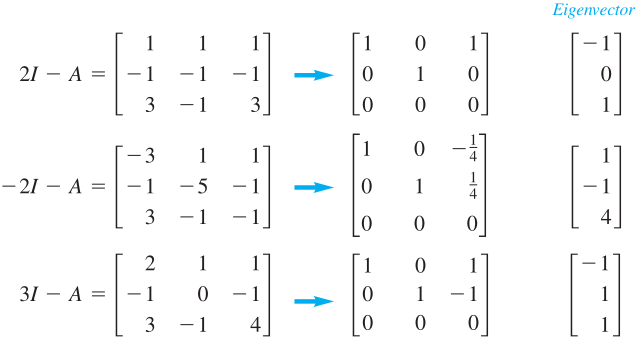
\includegraphics[width = 10cm]{images/unknown.png}
    \end{center}
    Form the matrix $P$ whose columns are the eigenvectors just obtained.
    \[P = \begin{bmatrix}[rrr]
        -1 & 1 & -1\\
        0 & -1 & 1\\
        1 & 4 & 1
    \end{bmatrix} \quad \text{and} \quad P^{-1} = \begin{bmatrix}[rrr]
        -1 & -1 & 0 \\
        \frac{1}{5} & 0 & \frac{1}{5} \\
        \frac{1}{5} & 1 & \frac{1}{5}
    \end{bmatrix}  \]
    So, $B = \{(-1,0,1), (1,-1,4),(-1,1,1) \}$. The matrix $T$ relative to this basis is
    \[D = P^{-1}AP = \begin{bmatrix}[rrr]
        2 & 0 & 0 \\
        0 & -2 & 0 \\
        0 & 0 & 3
    \end{bmatrix} \]

    \section{Symmetric Matrices and Orthogonal Diagonalization}
    Most matrices requires much of diagonaliation process before we can finally determine whether it is possible. One
    exception is a triangular matrix with distinct entries on the main diagonal. In this section, we will study 
    another type of matrix that is guaranteed to be \textbf{diagonalizable} - a \textbf{symmetric} matrix.
    \begin{Def}[Symmetric Matrix]
       A square matrix $A$ is \textbf{symmetric} if it is equal to its transpose:
       \[A = A^T\]
    \end{Def}
    \begin{tcolorbox}[colback = {blue9}]
        \textit{THEOREM 7.7} \textbf{Eigenvalues of Symmetric Matrices}

        If $A$ is an $n \times n$ symmetric matrix, then the following properties are true.\\
        1. $A$ is diagonalizable.\\
        2. All eigenvalues of $A$ are real.\\
        3. If $ \lambda $ is an eigenvalue of $A$ with multiplicity $k$,then $ \lambda $ has $k$ linearly independent eigenvectors.
        That is, the eigenspace of $ \lambda $ has dimension $k$.
    \end{tcolorbox}
    \textbf{REMARK.} The Theorem 7.7 is called the \textbf{Real Spectral Theorem}, and the set of eigenvalues of $A$ is called the \textbf{spectrum}
    of $A$.

    \textbf{Example 2. \textcolor{blue5}{The Eigenvalues and Eigenvectors of a 2 $\times$ 2 Symmetric Matrix}}

    Prove that $A = \begin{bmatrix}[cc]
        a & c \\
        c & b
    \end{bmatrix}$ is diagonalizable.

    \textit{\textcolor{blue5}{SOLUTION.}} The characteristic polynomial of $A$ is 
    \[| \lambda I - A| = \begin{vmatrix}
        \lambda  - a & -c \\
        -c & \lambda -b 
    \end{vmatrix}  = \lambda ^2 - (a+b) \lambda  + ab - c^2 \]
    As a quadratic in $ \lambda $, this polynomial has a discriminant of
    \begin{equation*}
        \begin{split}
            (a+b)^2 - 4(ab - c^2) &= a^2 + 2ab + b^2 - 4ab + 4c^2 \\
                                  &= (a-b)^2 + 4c^2 \ge 0
        \end{split}
    \end{equation*}
    $\bullet$ If $\Delta = 0 \implies a = b, c = 0$, which implies that $A$ is already diagonal.
    $\bullet$ If $\Delta > 0$, $A$ has 2 distinct real eigenvalues, then $A$ is diagonalizable also.

    \textbf{Example 5. \textcolor{blue5}{Dimension of the Eigenspaces of a Symmetric Matrix}}

    Find the eigenvalues of the symmetric matrix
    \[A = \begin{bmatrix}[rrrr]
        1 & -2 & 0 & 0\\
        -2 & 1 & 0 & 0\\
        0 & 0 & 1 & -2\\
        0 & 0 & -2 & 1
    \end{bmatrix} \]
    and determine the dimensions of the corresponding eigenspaces.

    \textit{\textcolor{blue5}{SOLUTION.}} The characteristic polynomial of $A$ is represented by
    \[| \lambda I - A| = \begin{vmatrix}[rrrr]
        \lambda  - 1 & 2 & 0 & 0 \\
        2 & \lambda  - 1 & 0 & 0 \\
        0 & 0 & \lambda  - 1 & 2 \\
        0 & 0 & 2 & \lambda  - 1
    \end{vmatrix} = ( \lambda  + 1 )^2( \lambda  - 3 )^2\]
    So, the eigenvalues are $ \lambda _1 = -1$ and $ \lambda _2 = 3$, which all have a multiplicity of $2$, so the corresponding
    eigenspaces also have dimensions 2.

    \section{Orhogonal Matrices}
    To diagonalize a matrix $A$, we need to find $P$ (\textit{invertible}) such that $P^{-1}AP$ is diagonal. For \textbf{symmetric} matrices,
    $P$ can be chosen to have a special properties.
    \begin{Def}[Orthogonal Matrix]
        A square matrix $P$ is called \textbf{orthogonal} if it is invertible and if
        \[P^{-1} = P^T\]
    \end{Def}
    
    \begin{tcolorbox}[colback = {blue9}]
        \textit{THEOREM 7.8} \textbf{Property of Orthogonal Matrices}

        An $n \times n$ matrix $P$ is orthogonal if and only if its column vectors form an \textbf{orthonormal} set.
    \end{tcolorbox}

    \textit{\textcolor{blue5}{PROOF}}  Suppose the column vectors of $P$ form an orthonormal set. (p.469)
    
    \textbf{Example 5. \textcolor{blue5}{An Orthogonal Matrix}}

    Show that 
    \[P = \begin{bmatrix}[rrr]
        \frac{1}{3} & \frac{2}{3} & \frac{2}{3}\\
        - \frac{2}{\sqrt{5}} & \frac{1}{\sqrt{5}} & 0\\
        - \frac{2}{3\sqrt{5}} & - \frac{4}{3\sqrt{5}} & \frac{5}{3\sqrt{5}}
    \end{bmatrix} \]
    is orthogonal by showing that $PP^T = 1$. Then show that the column vectors of $P$ form an orthonormal set.

    \textit{\textcolor{blue5}{SOLUTION.}} $PP^T = 1$, we can conclude that $P$ is orthogonal.

    Moreover, letting
    \[ \textbf{p}_1 = \begin{bmatrix}[r]
        \frac{1}{3}\\
        - \frac{2}{\sqrt{5}} \\
        - \frac{2}{3\sqrt{5}}
    \end{bmatrix} , \quad \textbf{p}_2 = \begin{bmatrix}[r]
        \frac{2}{3} \\
        \frac{1}{\sqrt{5}} \\
        - \frac{4}{3\sqrt{5}}
    \end{bmatrix} , \quad \text{and } \textbf{p}_3 = \begin{bmatrix}[r]
        \frac{2}{3}\\
        0\\
        \frac{5}{3\sqrt{5}}
    \end{bmatrix} \]
    produces
    \[ \textbf{p}_1 \cdot \textbf{p}_2 = \textbf{p}_2 \cdot \textbf{p}_3 = \textbf{p}_3 \cdot \textbf{p}_1 = 0\]
    and 
    \[\norm{ \textbf{p}_1 } = \norm{ \textbf{p}_2 } = \norm{ \textbf{p}_3 } = 1\]

    \begin{tcolorbox}[colback = {blue9}]
        \textit{THEOREM 7.9} \textbf{Property of Symmetric Matrices}

        Let $A$ be an $n \times n$ symmetric matrix. If $ \lambda _1$ and $ \lambda _2$ are 2 distinct eigenvalues of $A$, then their corresponding 
        eigenvectors $ \textbf{x}_1$ and $ \textbf{x}_2$ are \textbf{orthogonal}.
    \end{tcolorbox}
    \textit{\textcolor{blue5}{PROOF}}  (p471)

    \section{Orthogonal Diagonalization}
    A matrix $A$ is \textbf{orthogonally diagonalizable} if there exists an orthogonal matrix $P$ such that 
    $P^{-1}AP = D$ is diagonal.
    \begin{tcolorbox}[colback = {blue9}]
        \textit{THEOREM 7.10} \textbf{Fundamental Theorem of Symmetric Matrices}

        Let $A$ be an $n \times n$ matrix. Then $A$ is \textbf{orthogonally diagonalizable} and has real eigenvalues if and only if
        $A$ is \textbf{symmetric}.
    \end{tcolorbox}
    \textit{\textcolor{blue5}{PROOF}} (p472) 

    \textbf{Example 7. \textcolor{blue5}{Determining Whether a Matrix is Orthogonally Diagonalizable}}

    Just choose the \textbf{symmetric} ones.

    \begin{tcolorbox}[colback = {blue9}]
        \textbf{Orthogonal Diagonalization of a Symmetric Matrix}

        Let $A$ be an $n \times n$ symmetric matrix.\\
        1. Find all eigenvalues of $A$ and determine the multiplicity of each.\\
        2. \textbf{Normalize} the eigenvectors, make every set \textbf{orthonormal}. (Applying the Gram-Schmidt o.p) \\
        4. Use $n$ eigenvectors to form the columns of $P$. The matrix $D = P^{-1}AP = P^TAP$ is diagonal.
    \end{tcolorbox}

    \textbf{Example 8. \textcolor{blue5}{Orthogonal Diagonalization}}

    Find an orthogonal matrix $P$ that orthogonally diagonalizes
    \[A = \begin{bmatrix}[rr]
        -2 & 2 \\
        2 & 1
    \end{bmatrix} \]

    \textit{\textcolor{blue5}{SOLUTION.}} The characteristic polynomial of $A$ is
    \[| \lambda I - A| = \begin{vmatrix}[rr]
        \lambda  + 2 & -2 \\
        -2 & \lambda  - 1
    \end{vmatrix} = ( \lambda  + 3 )( \lambda  - 2 )\]
    So, the eigenvalues are $ \lambda _1 = -3$ and $ \lambda _2 = 2$. For each of those, find an eigenvector by converting the matrix
    $| \lambda I - A$ to reduced row-echelon form.
    
    \begin{align*}
        & & -3I - A & & = & &\begin{bmatrix}[rr]
            -1 & -2\\
            -2 & -4
            \end{bmatrix}&  & \implies & & \begin{bmatrix}[rr]
        1 & 2 \\ 
        0 & 1
        \end{bmatrix}&  & \implies & & \begin{bmatrix}[rr]
        -2 \\ 1
    \end{bmatrix} & & \\
        & & 2I - A & & = & &\begin{bmatrix}[rr]
                4 & -2 \\
                -2 & 1
            \end{bmatrix}& & \implies & &
                \begin{bmatrix}[rr]
                    1 & - \frac{1}{2} \\
                    0 & 0 
                    \end{bmatrix}& & \implies & &\begin{bmatrix}[cc]
                    1 \\ 2
                \end{bmatrix} & &
    \end{align*}
    Normalize these eigenvectors to produce an \textit{orthonormal} basis.
    \begin{equation*}
        \begin{split}
            \textbf{p}_1 &= \ddfrac{(-2,1)}{\norm{(-2,1)}} = \ddfrac{1}{\sqrt{5}} (-2,1) = \left( - \ddfrac{2}{\sqrt{5}} , \ddfrac{1}{\sqrt{5}}\right) \\
            \textbf{p}_2 &= \ddfrac{(1,2)}{\norm{(1,2)}} = \ddfrac{1}{\sqrt{5}} (1,2) = \left( \ddfrac{1}{\sqrt{5}} , \ddfrac{2}{\sqrt{5}}  \right)
        \end{split}
    \end{equation*} 
    Using $ \textbf{p}_1$ and $ \textbf{p}_2$ as column vectors, construct the matrix $P$.
    \[P = \begin{bmatrix}[rr]
        - \frac{2}{\sqrt{5}} & \frac{1}{\sqrt{5}} \\
        \frac{1}{\sqrt{5}} & \frac{2}{\sqrt{5}} 
    \end{bmatrix} \]
    \pagebreak
    
    \textbf{Example 9. \textcolor{blue5}{Orthogonal Diagonalization}}

    Find an orthogonal matrix $P$ that diagonalizes 
    \[A = \begin{bmatrix}[rrr]
        2 & 2 & -2\\
        2 & -1 & 4\\
        -2 & 4 & -1
    \end{bmatrix} \]

    \textit{\textcolor{blue5}{SOLUTION.}} The characteristic polynomial of $A$, $| \lambda I - A| = ( \lambda  - 3 )^2( \lambda  + 6 )$ yields the 
    eigenvalues $ \lambda _1 = -6$ (multiplicity of 1) and $ \lambda _2 = 3$ (multiplicity of 2). 

    $\bullet$ For $ \lambda _1 = -6$, an eigenvector is $ \textbf{v}_1 = (1, -2, 2)$, which normalizes to
    \[ \textbf{u}_1 = \frac{ \textbf{v}_1 }{\norm{ \textbf{v}_1 }} = \left( \frac{1}{3}, - \frac{2}{3}, \frac{2}{3} \right) \]
    $\bullet$ For $ \lambda _2 = 3$, 2 eigenvectors are $ \textbf{v}_2 = (2,1,0)$ and $ \textbf{v}_3 = (-2,1,0)$. Note that $ \textbf{v}_1$ is 
    \textit{orthogonal} to them, but these 2 are \textbf{not} orthogonal. Applying the Gram-Schmidt process:
    \begin{equation*}
        \begin{split}
            \textbf{u}_2 &= \ddfrac{\textbf{w}_2}{\norm{\textbf{w}_2}} = \ddfrac{1}{\sqrt{5}} (2,1,0) = \left( \ddfrac{2}{\sqrt{5}} , \ddfrac{1}{\sqrt{5}} , 0 \right)\\
            \textbf{u}_3 &= \ddfrac{\textbf{w}_3}{\norm{\textbf{w}_3}} = \ddfrac{3\sqrt{5}}{5} \left(- \ddfrac{2}{5} , \ddfrac{4}{5} ,1 \right) 
            = \left( - \ddfrac{2}{3\sqrt{5}} , \ddfrac{4}{3\sqrt{5}} , \ddfrac{5}{3\sqrt{5}}  \right)
        \end{split}
    \end{equation*}
    Form the matrix $P$:
    \[P = \begin{bmatrix}[rrr]
        \frac{1}{3} & \frac{2}{\sqrt{5}} & - \frac{2}{3\sqrt{5}} \\
        - \frac{2}{3} & \frac{1}{\sqrt{5}} & \frac{4}{3\sqrt{5}}\\
        \frac{2}{3} &  0 & \frac{5}{3\sqrt{5}}
    \end{bmatrix} \]


\end{document}
